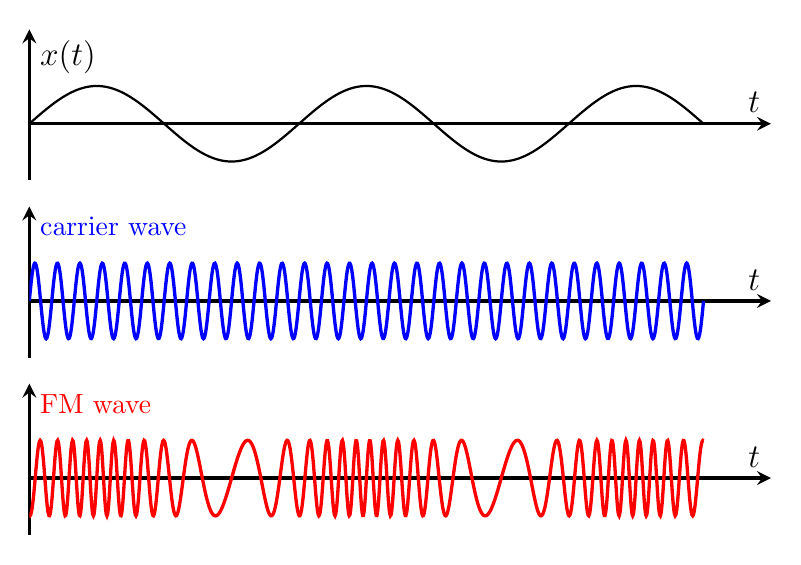
\begin{tikzpicture}[samples=1000, domain=0:10]

	\begin{axis}[
		width=11cm, height=3.5cm,
		xtick=\empty,
		ytick=\empty,
		xlabel={\large $t$},
		ylabel={\large $x(t)$},
		xmin=0, xmax=11,
		ymin=-3, ymax=5,
		axis lines = middle,
		very thick,
		trig format = rad
	]
		\addplot [no markers, smooth, thick] {2*sin(2*pi*0.25*x)};
	\end{axis}

	\begin{axis}[
		at={(0, -2.25cm)},
		width=11cm, height=3.5cm,
		xtick=\empty,
		ytick=\empty,
		xlabel={\large $t$},
		ylabel={\textcolor{blue}{carrier wave}},
		xmin=0, xmax=11,
		ymin=-3, ymax=5,
		axis lines = middle,
		very thick,
		trig format = rad
	]
		\addplot [no markers, smooth, blue, very thick] {2*sin(6*pi*x)};
	\end{axis}

	\begin{axis}[
		at={(0, -4.5cm)},
		width=11cm, height=3.5cm,
		xtick=\empty,
		ytick=\empty,
		xlabel={\large $t$},
		ylabel={\textcolor{red}{FM wave}},
		xmin=0, xmax=11,
		ymin=-3, ymax=5,
		axis lines = middle,
		very thick,
		trig format = rad
	]
		\addplot expression [no markers, smooth, red, very thick] {2*sin(2*pi*3*x - 8*cos(2*pi*0.25*x))};
	\end{axis}

\end{tikzpicture}

%Local variables:
% coding: utf-8
% mode: text
% mode: rst
% End:
% vim: fileencoding=utf-8 filetype=tex :
